\documentclass[10pt,twocolumn]{article}

% --- Packages ---
\usepackage[margin=0.75in]{geometry}
\usepackage{amsmath}
\usepackage{amssymb}
\usepackage{graphicx}
\usepackage{booktabs}
\usepackage{array}
\usepackage{tabularx}
\usepackage{tikz}
\usetikzlibrary{arrows.meta,positioning,shapes.geometric,fit}
\usepackage{hyperref}
\usepackage{caption}
\usepackage{subcaption}
\usepackage{xcolor}
\usepackage{listings}
\usepackage{float}

% --- Listings style for ASCII art / code ---
\lstset{
  basicstyle=\ttfamily\scriptsize,
  breaklines=true,
  frame=none,
  columns=fullflexible,
  keepspaces=true,
}

% --- Table helpers ---
\newcolumntype{Y}{>{\raggedright\arraybackslash}X}
\newcolumntype{Z}{>{\centering\arraybackslash}X}

% --- Hyperref setup ---
\hypersetup{
  colorlinks=true,
  linkcolor=blue!60!black,
  citecolor=green!50!black,
  urlcolor=blue,
}

% --- Title block ---
\title{\textbf{Parametric Weapon Design Optimisation: A Comparison of Spline
Profile Families with FEA-in-Loop Evaluation}}

\author{[Author]}

\date{\today}

% =============================================================================
\begin{document}
\maketitle

% =============================================================================
\begin{abstract}
We present a modular optimisation framework for the automated design of combat robot spinning weapons.  The system exposes five independent modules: Profile, Cutout, Objective, Optimizer, and FEA Eval. Each can be configured independently and <modularly swapped>. Three spline profile families are compared: a periodic cubic B-spline, a composite cubic B\'ezier, and a centripetal Catmull-Rom spline. A frozen Fourier radial series serves as the baseline. Weight-reduction pockets are modelled as superelliptic cutouts parameterised in polar coordinates.  The enhanced objective replaces formula-constant bite depth with a kinematic Archimedean spiral simulation and replaces a geometric structural proxy with coarse-mesh 2D plane-stress FEA evaluated inside the optimisation loop.  Differential evolution drives a two-phase search over $N{=}12$ radial control points (Phase~1) and up to six polar cutout parameters (Phase~2).  Preliminary results on four weapon archetypes show that the B-spline family converges most reliably, while centripetal Catmull-Rom yields the most interpretable parameter space.
\end{abstract}

% =============================================================================
\section{Introduction}
\label{sec:intro}

Combat robot competitions demand spinning weapons that maximise stored kinetic
energy, deliver large bite depth per tooth engagement, survive centrifugal and
impact stresses, and remain within strict mass and envelope rules.  Manual
design of these weapons is iterative and heavily experience-dependent; even
expert builders rely on trial-and-error tuning of shape parameters whose
interactions are poorly understood.

Automated optimisation of weapon geometry has the potential to explore the full
design space systematically and to make engineering trade-offs explicit.
However, the utility of any optimisation study depends critically on the
fidelity of the models used: a bite-depth formula that is constant for a given
RPM and style cannot reward geometry that genuinely increases engagement, and a
geometric structural proxy cannot detect stress concentrations introduced by
weight-relief pockets.

This paper describes a research comparison framework built around five
independently selectable \emph{swap points}.  The \emph{baseline} stack
(frozen, unmodified) uses a Fourier radial profile, elliptic Fourier cutouts, a
formula-constant bite model, and a geometric structural proxy---mirroring
prior practice.  The \emph{enhanced} stack replaces each component in turn: a
periodic B-spline (or B\'ezier, or Catmull-Rom) outer profile, polar
superelliptic cutouts, a kinematic spiral bite simulation, and coarse-mesh FEA
evaluated at every objective call.  All results are compared side-by-side via
\texttt{evaluate.py --mode compare}.

% =============================================================================
\section{System Architecture}
\label{sec:arch}

\subsection{Swap Points}
\label{sec:swappoints}

The optimisation stack is built from five independently configurable components,
each governed by a field in the \texttt{OptimizationParams} dataclass.
Table~\ref{tab:swappoints} lists the swap points, their interface contracts,
the available implementations, and the controlling config key.

\begin{table}[t]
  \caption{Swap-point summary (see also \texttt{docs/ARCHITECTURE.md}).}
  \label{tab:swappoints}
  \footnotesize
  \begin{tabular}{@{}p{0.18\linewidth} p{0.22\linewidth} p{0.40\linewidth} p{0.16\linewidth}@{}}
    \toprule
    \textbf{Slot} & \textbf{Interface} & \textbf{Implementations} &
    \textbf{Config} \\
    \midrule
    Profile   & radii $\to$ poly
              & fourier; bspline; bezier; catmull
              & profile\_type \\
    Cutout / P2
              & poly $\to$ poly+holes
              & fourier ellipses; superellipse pockets; topology (SIMP)
              & cutout\_type \\
    Objective & poly $\to$ metrics
              & baseline (formula + geometric proxy); enhanced (spiral bite + FEA)
              & evaluation\_mode \\
    Optimizer & cfg $\to$ run
              & baseline DE; enhanced DE
              & evaluation\_mode \\
    FEA       & poly $\to$ fea score
              & off; coarse; fine; spiral contact loads (post-hoc)
              & fea\_interval \\
    \bottomrule
  \end{tabular}
\end{table}

\subsection{Data Flow}
\label{sec:dataflow}

A single enhanced-mode evaluation follows the pipeline in
Figure~\ref{fig:dataflow}.  The \texttt{WeaponConfig} is the single root
object; every component reads only the fields it needs.

\begin{figure}[H]
  \centering
  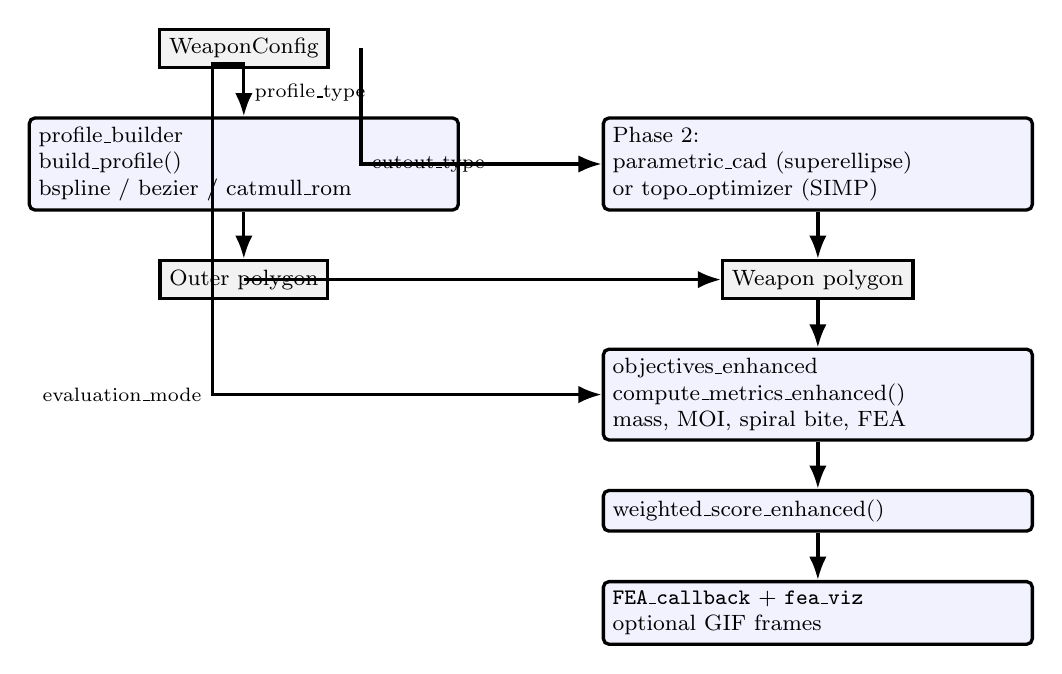
\begin{tikzpicture}[
    node distance=6mm and 10mm,
    proc/.style={rectangle, rounded corners=2pt, draw, very thick, fill=blue!5, align=left, text width=0.43\linewidth, font=\footnotesize},
    data/.style={rectangle, draw, very thick, fill=gray!10, align=center, font=\footnotesize, minimum width=18mm},
    arrow/.style={-Latex, very thick}
  ]
    \node[data] (cfg) {WeaponConfig};
    \node[proc, below=of cfg] (profile) {profile\_builder\\build\_profile()\\bspline / bezier / catmull\_rom};
    \node[data, below=of profile] (outer) {Outer polygon};
    \node[proc, right=18mm of profile] (cutout) {Phase 2:\\parametric\_cad (superellipse)\\or topo\_optimizer (SIMP)};
    \node[data, below=of cutout] (weapon) {Weapon polygon};
    \node[proc, below=of weapon] (metrics) {objectives\_enhanced\\compute\_metrics\_enhanced()\\mass, MOI, spiral bite, FEA};
    \node[proc, below=of metrics] (score) {weighted\_score\_enhanced()};
    \node[proc, below=of score] (fea) {\texttt{FEA\_callback} + \texttt{fea\_viz}\\optional GIF frames};

    \draw[arrow] (cfg) -- node[right, font=\scriptsize]{profile\_type} (profile);
    \draw[arrow] (profile) -- (outer);
    \draw[arrow] (cfg.east) ++(0.4,0) |- node[right, font=\scriptsize]{cutout\_type}(cutout);
    \draw[arrow] (cutout) -- (weapon);
    \draw[arrow] (outer) |- (weapon);
    \draw[arrow] (cfg) |- ++(-0.4,-0.2) |- node[left, font=\scriptsize]{evaluation\_mode} (metrics);
    \draw[arrow] (weapon) -- (metrics);
    \draw[arrow] (metrics) -- (score);
    \draw[arrow] (score) -- (fea);
  \end{tikzpicture}
  \caption{Enhanced-mode data flow (WeaponConfig driven).}
  \label{fig:dataflow}
\end{figure}

Recent code updates (see \texttt{ARCHITECTURE.md}) add two notable options not
present in the original draft: (i) \texttt{cutout\_type = topology}, which
replaces Phase~2 DE pockets with a SIMP topology optimisation loop; and
(ii) optional spiral contact force injection into FEA for post-hoc stress
studies.  The data-flow diagram above already includes both paths.

\subsection{Permutation Matrix}
\label{sec:permmatrix}

Table~\ref{tab:permmatrix} lists the valid slot combinations.  The first row is
the frozen baseline used as the research reference; all other rows are enhanced
variants explored in this work.

\begin{table}[H]
  \caption{Valid slot combinations (see \texttt{docs/ARCHITECTURE.md}).}
  \label{tab:permmatrix}
  \footnotesize
  \begin{tabular}{@{}p{0.17\linewidth} p{0.19\linewidth} p{0.14\linewidth} p{0.12\linewidth} p{0.30\linewidth}@{}}
    \toprule
    \textbf{Profile} & \textbf{Cutout} & \textbf{Obj.} & \textbf{FEA}
      & \textbf{Description} \\
    \midrule
    fourier      & fourier      & baseline & off    & Frozen baseline \\
    bspline      & superellipse & enhanced & coarse & Enhanced default \\
    bspline      & topology     & enhanced & coarse & SIMP Phase~2 \\
    bezier       & superellipse & enhanced & coarse & Bézier variant \\
    catmull\_rom & superellipse & enhanced & coarse & Catmull-Rom variant \\
    any spline   & superellipse or topology & enhanced & fine & Hi-res FEA/GIF \\
    bspline      & fourier      & enhanced & off    & Legacy cutouts \\
    \bottomrule
  \end{tabular}
\end{table}

% =============================================================================
\section{Profile Parametrisations}
\label{sec:profiles}

All four profile families share the same interface:
\begin{equation}
  f(\boldsymbol{r},\, R_{\max},\, R_{\min},\, n_{\mathrm{eval}})
  \;\longrightarrow\; \text{Polygon} \mid \texttt{None}
\end{equation}
where $\boldsymbol{r} = [r_0, r_1, \ldots, r_{N-1}]$ is the vector of $N$
radial control values in millimetres, one at each uniformly-spaced angle
$\theta_i = 2\pi i/N$.  All radii are clamped to $[R_{\min}, R_{\max}]$ before
evaluation.  The output is a closed Shapely \texttt{Polygon} with
$n_{\mathrm{eval}}$ vertices ($n_{\mathrm{eval}} = 360$ by default).

\subsection{Fourier Radial Series (baseline, frozen)}
\label{sec:fourier}

The baseline profile is a Fourier radial series:
\begin{equation}
  R(\theta) = R_{\mathrm{base}}
    + \sum_{k=1}^{K}\bigl(a_k \cos k\theta + b_k \sin k\theta\bigr)
  \label{eq:fourier}
\end{equation}
where $R_{\mathrm{base}}$ is the mean radius and the $2K$ coefficients
$(a_k, b_k)$ are the optimisation variables.  The profile is evaluated at
$n_{\mathrm{eval}}$ equally-spaced angles and wrapped into a polygon.

The Fourier series is implemented in \texttt{parametric.py} and is frozen for
the duration of this study.  Its main limitation is that every coefficient
affects the entire profile (\emph{global support}), so small perturbations to
one coefficient can propagate oscillations around the whole weapon.  Additionally,
abrupt changes between optimiser steps can excite high-frequency Gibbs-type
ringing when $K$ is moderate and the target profile has sharp features.

\subsection{Periodic Cubic B-Spline}
\label{sec:bspline}

The B-spline profile replaces the frequency-domain parameters with $N$
radial control values at uniformly-spaced angles:
\begin{equation}
  \theta_i = \frac{2\pi i}{N}, \quad i = 0,\ldots,N-1
\end{equation}
Control point $i$ is placed at
$(r_i \cos\theta_i,\; r_i \sin\theta_i)$.
A periodic cubic B-spline is then fitted through these $N$ Cartesian control
points using \texttt{scipy.interpolate.splprep} with \texttt{per=True} and
\texttt{k=3} (cubic, $s{=}0$ interpolating).  The spline is evaluated at
$n_{\mathrm{eval}}$ uniformly-spaced parameter values $u \in [0, 1)$ to
produce the polygon vertices.

\paragraph{Properties.}
The periodic B-spline satisfies C\textsuperscript{2} continuity everywhere
by construction.  Because the underlying B-spline basis has \emph{local
support} of width $4/N$ in parameter space, moving a single control radius
$r_i$ affects the profile only in the angular neighbourhood
$[\theta_i - 4\pi/N,\; \theta_i + 4\pi/N]$, not the full weapon outline.
No Gibbs phenomenon occurs because the spline degree is fixed at three
regardless of $N$.  The control radii are directly interpretable: $r_i$ is
(approximately) the weapon radius at angle $\theta_i$.

\subsection{Composite Cubic B\'ezier}
\label{sec:bezier}

The composite B\'ezier profile uses $N$ cubic B\'ezier segments joined at
the $N$ control points, yielding a closed curve with C\textsuperscript{1}
continuity at each join.  Tangents are computed via Catmull-Rom-style
central differences:
\begin{equation}
  \boldsymbol{T}_i = \tfrac{1}{2}\!\left(\boldsymbol{P}_{i+1} - \boldsymbol{P}_{i-1}\right)
  \label{eq:cr_tangent}
\end{equation}
with periodic (modular) index arithmetic.  For segment $i$ from
$\boldsymbol{P}_i$ to $\boldsymbol{P}_{i+1}$, the four B\'ezier control points
are:
\begin{align}
  \boldsymbol{C}_{1,i} &= \boldsymbol{P}_i + \tfrac{1}{3}\boldsymbol{T}_i \\
  \boldsymbol{C}_{2,i} &= \boldsymbol{P}_{i+1} - \tfrac{1}{3}\boldsymbol{T}_{i+1}
\end{align}
Each segment is evaluated using the standard cubic B\'ezier formula:
\begin{equation}
  \boldsymbol{B}(t) = (1{-}t)^3\boldsymbol{P}_i
    + 3(1{-}t)^2 t\,\boldsymbol{C}_{1,i}
    + 3(1{-}t)t^2\boldsymbol{C}_{2,i}
    + t^3\boldsymbol{P}_{i+1}
\end{equation}

\paragraph{Properties.}
C\textsuperscript{1} continuity (matched tangents, possible curvature
discontinuity at joins).  Each segment is controlled by exactly two adjacent
control points plus their neighbours---tighter local support than the
B-spline.  The parameter space is identical to the B-spline: $N$ radii at
equally-spaced angles.

\subsection{Centripetal Catmull-Rom}
\label{sec:catmullrom}

The centripetal Catmull-Rom profile uses the Barry-Goldman recursive algorithm
to evaluate a closed Catmull-Rom spline with parameterisation exponent
$\alpha = 0.5$.  For each segment $i$, four control points are used:
$(\boldsymbol{P}_{i-1}, \boldsymbol{P}_i, \boldsymbol{P}_{i+1}, \boldsymbol{P}_{i+2})$
with periodic wrapping.

The centripetal knot sequence is:
\begin{equation}
  t_0 = 0, \quad
  t_{k+1} = t_k + \|\boldsymbol{P}_{k+1} - \boldsymbol{P}_k\|^{\alpha}
\end{equation}
The local parameter $t \in [0,1]$ is remapped to $[t_1, t_2]$ for each
segment.  The Barry-Goldman algorithm computes the Catmull-Rom point via
two levels of linear interpolation:
\begin{align}
  A_j &= \mathrm{lerp}(\boldsymbol{P}_{j-1}, \boldsymbol{P}_j;\; t_{j-1}, t_j,\; t) \\
  B_j &= \mathrm{lerp}(A_j, A_{j+1};\; t_{j-1}, t_{j+1},\; t) \\
  \boldsymbol{C}(t) &= \mathrm{lerp}(B_1, B_2;\; t_1, t_2,\; t)
\end{align}

\paragraph{Properties.}
Unlike the B-spline and B\'ezier families, the Catmull-Rom spline
\emph{interpolates} every control point: the curve passes exactly through
$(r_i \cos\theta_i,\; r_i \sin\theta_i)$ for all $i$.  This makes the parameter
space maximally interpretable---$r_i$ is the exact weapon radius at angle
$\theta_i$.  The centripetal variant ($\alpha{=}0.5$) spaces knots
proportionally to $\sqrt{\|\Delta\boldsymbol{P}\|}$, preventing cusps and
self-intersections that the uniform variant ($\alpha{=}0$) can produce for
widely-spaced or non-uniform control points.  Continuity is C\textsuperscript{1}.

\subsection{Profile Family Comparison}
\label{sec:profilecomp}

Table~\ref{tab:profilecomp} summarises the key properties of each family.

\begin{table}[H]
  \caption{Profile parametrisation comparison.}
  \label{tab:profilecomp}
  \small
  \begin{tabularx}{\linewidth}{@{}l Z Z Z Z@{}}
    \toprule
    \textbf{Family} & \textbf{Cont.} & \textbf{Local} & \textbf{Interp.}
      & \textbf{Gibbs} \\
    \midrule
    Fourier         & C$^\infty$ & No  & No  & Yes \\
    B-spline        & C$^2$      & Yes & No  & No  \\
    Bezier          & C$^1$      & Yes & No  & No  \\
    Catmull-Rom     & C$^1$      & Yes & Yes & No  \\
    \bottomrule
    \multicolumn{5}{@{}l@{}}{\footnotesize Cont.~=~continuity order;
      Local~=~local support; Interp.~=~interpolates control points.}
  \end{tabularx}
\end{table}

% =============================================================================
\section{Evaluation Methods}
\label{sec:eval}

\subsection{Baseline Objective}
\label{sec:baseline_obj}

The baseline objective, implemented in \texttt{objectives.py}, computes a
weighted sum of five sub-scores:

\begin{equation}
  S_{\mathrm{base}} = w_1 E + w_2 B + w_3 \mathit{IZ} + w_4 \mathit{Str} + w_5 \mathit{Sym}
\end{equation}

where $E$ is stored kinetic energy (from \texttt{physics.stored\_energy\_joules}),
$B$ is bite depth from the formula model, $\mathit{IZ}$ is the impact zone score,
$\mathit{Str}$ is the structural score, and $\mathit{Sym}$ is a symmetry
penalty.

\paragraph{Formula bite.}
Bite depth in the baseline is computed by \texttt{bite\_mm()} in
\texttt{physics.py}:
\begin{equation}
  b = \frac{v_{\mathrm{approach}}}{n_{\mathrm{teeth}} \cdot f_{\mathrm{rot}}}
\end{equation}
where $v_{\mathrm{approach}}$ is the closing speed (m/s), $n_{\mathrm{teeth}}$
is a \emph{hardcoded} integer per weapon style (1, 2, or 3), and
$f_{\mathrm{rot}}$ is the rotation frequency (Hz).  Because
$n_{\mathrm{teeth}}$ is not derived from the weapon geometry, the optimiser
cannot increase the score by modifying the number or prominence of teeth.

\paragraph{Geometric structural proxy.}
The structural score in \texttt{structural.py} uses minimum wall thickness
and the section width at the bore as a proxy for bending stiffness.  No FEA
is performed during baseline optimisation.

\subsection{Enhanced Objective: Kinematic Spiral Bite}
\label{sec:spiral}

The enhanced objective, implemented in \texttt{objectives\_enhanced.py},
replaces the formula bite model with a kinematic simulation of tooth
engagement.

\paragraph{Physical model.}
In the weapon's rotating reference frame, the approaching enemy robot's face
traces an Archimedean spiral.  Let $\omega = 2\pi \cdot \mathrm{RPM}/60$\,rad/s
be the weapon angular velocity and $v$\,mm/s be the enemy closing speed.  The
radial advance per radian of weapon rotation is:
\begin{equation}
  v_{\mathrm{rad}} = \frac{v}{\omega}
  \quad [\text{mm/rad}]
\end{equation}

The enemy's position in the rotating frame is modelled as an Archimedean spiral:
\begin{equation}
  r_{\mathrm{enemy}}(\theta) = r_{\mathrm{start}} - v_{\mathrm{rad}} \cdot \theta
  \label{eq:spiral}
\end{equation}
where $r_{\mathrm{start}}$ is the initial standoff distance and $\theta$ is
the cumulative weapon rotation angle over one revolution.

\paragraph{Contact counting.}
The weapon's radial profile $r_{\mathrm{profile}}(\theta)$ is sampled at 720
equally-spaced angles.  A contact event occurs at each zero-crossing where
the spiral transitions from outside to inside the profile:
\begin{equation}
  r_{\mathrm{enemy}}(\theta_k) > r_{\mathrm{profile}}(\theta_k)
  \;\;\text{and}\;\;
  r_{\mathrm{enemy}}(\theta_{k+1}) \leq r_{\mathrm{profile}}(\theta_{k+1})
\end{equation}
Let $n_{\mathrm{contacts}}$ be the number of such crossings per revolution.

\paragraph{Effective bite depth.}
The bite depth (enemy advance between consecutive contacts) is:
\begin{equation}
  b_{\mathrm{eff}} = \frac{v_{\mathrm{rad}} \cdot 2\pi}{n_{\mathrm{contacts}}}
  \label{eq:bite}
\end{equation}

This correctly incentivises fewer, more pronounced protrusions:
\begin{itemize}
  \item A smooth disk: $n_{\mathrm{contacts}} = 1$, maximum bite
    $\approx 22.5$\,mm at 8000\,RPM and 3\,m/s closing speed.
  \item Twelve small teeth: $n_{\mathrm{contacts}} \approx 12$, bite reduced
    to $\approx 1/12$ of maximum.
\end{itemize}

\subsection{FEA-in-Loop Structural Scoring}
\label{sec:fea}

The enhanced stack replaces the geometric structural proxy with a 2D
constant-strain triangle (CST) plane-stress finite element analysis, implemented
in \texttt{fea.py}.

\paragraph{Problem formulation.}
The weapon polygon is discretised into a triangular mesh with spacing
controlled by \texttt{fea\_coarse\_spacing\_mm} (default 10\,mm during
optimisation, 4\,mm for final renders).  The centrifugal body force per unit
area is:
\begin{equation}
  \boldsymbol{f}_c = \rho \omega^2 \boldsymbol{r}
\end{equation}
where $\rho$ is the material density (kg/mm\textsuperscript{2}),
$\omega$ is the angular velocity, and $\boldsymbol{r}$ is the position vector
from the rotation axis.  A fixed boundary condition is applied at all nodes
inside the bore circle.

\paragraph{Stress metric.}
The FEA returns per-element Von Mises stresses.  The structural score is
derived from the safety factor:
\begin{equation}
  \mathit{SF} = \frac{\sigma_{\mathrm{yield}}}{\sigma_{\mathrm{VM,max}}}
\end{equation}

High safety factors contribute positively to the objective; stress
concentrations at thin web sections near cutouts reduce the score.

\paragraph{Computational cost.}
At 10\,mm mesh spacing, a typical 150\,mm-radius disk weapon produces
approximately 200--400 elements, with each FEA solve taking 5--20\,ms on a
single CPU core.  With 200 optimiser iterations and a population of 15 per
differential evolution step, the total FEA budget is manageable on consumer
hardware.

% =============================================================================
\section{Optimisation Framework}
\label{sec:optim}

\subsection{Differential Evolution}
\label{sec:de}

Both baseline and enhanced stacks use SciPy's \texttt{differential\_evolution}
solver~\cite{storn1997de} with strategy \texttt{best1bin}.  The enhanced
optimizer (\texttt{optimizer\_enhanced.py}) runs a two-phase search; the
baseline optimizer runs a single phase.

\subsection{Phase 1: Outer Profile}
\label{sec:phase1}

Phase~1 optimises the $N_{\mathrm{bs}}$ B-spline (or B\'ezier, or
Catmull-Rom) control radii.  The search bounds for all control radii are
identical:
\begin{equation}
  r_i \in [R_{\min},\; R_{\max}], \quad i = 0, \ldots, N_{\mathrm{bs}}-1
\end{equation}
where $R_{\min} = \max(r_{\mathrm{bore}} + t_{\min} + 5, 15)$\,mm and
$R_{\max}$ is the envelope limit (or half-diagonal for bar-style weapons).
The default value is $N_{\mathrm{bs}} = 12$.

The Phase~1 objective is the full enhanced score with no cutouts: profile
only, with mass, energy, bite, and FEA terms.

Phase~1 uses 50\% of the total iteration budget.

\subsection{Phase 2: Polar Superellipse Cutouts}
\label{sec:phase2}

Phase~2 fixes the best profile from Phase~1 and optimises the weight-relief
pockets.  Each pocket is parameterised as a superellipse in polar coordinates:
\begin{equation}
  \left|\frac{x'}{a}\right|^n + \left|\frac{y'}{b}\right|^n \leq 1
\end{equation}
where $(x', y')$ are coordinates in a local frame centred at polar position
$(r, \phi)$ relative to the bore axis, $a$ and $b$ are the semi-axes, and
$n$ is the superellipse exponent ($n=2$ is an ellipse; $n=4$ gives a
rounded rectangle).  The five parameters $(r, \phi, a, b, n)$ per pocket are
optimised jointly for up to six pockets.

\paragraph{Mass normalisation.}
To decouple pocket shape from mass, an analytical normalisation step rescales
all semi-axes uniformly:
\begin{equation}
  s = \sqrt{\frac{A_{\mathrm{holes,target}}}{A_{\mathrm{holes,eff}}}}
\end{equation}
Iteration (up to three rounds) ensures the final weapon mass satisfies the
class limit to within 1\%.

Phase~2 uses 25\% of the total iteration budget.

\paragraph{Constraint handling.}
During Phase~2 the weapon is deliberately overweight (mass is fixed
analytically afterwards), so the mass constraint is excluded from the
constraint penalty.  A modified penalty function
\texttt{\_constraint\_penalty\_no\_mass()} is used for this purpose.

\subsection{Convergence Visualisation}
\label{sec:gif}

When \texttt{fea\_interval} $> 0$, the optimizer saves a sidecar triplet
every \texttt{fea\_interval} steps:
\begin{itemize}
  \item \texttt{frame\_NNNN.png} --- two-panel FEA stress map rendered at
    \texttt{fea\_fine\_spacing\_mm} resolution;
  \item \texttt{frame\_NNNN.npz} --- raw arrays (nodes, elements, Von Mises
    stresses, polygon geometry);
  \item \texttt{frame\_NNNN\_meta.json} --- step, phase, score, and full
    metrics dict.
\end{itemize}
After optimisation completes, \texttt{fea\_viz.export\_gif()} assembles
these frames into \texttt{convergence\_phase1.gif} and
\texttt{convergence\_phase2.gif}.  The sidecar format enables
\texttt{fea\_replay.py} to re-render GIFs post-hoc with different colour
scales or DPI without re-running the optimiser.

% =============================================================================
\section{Method Comparison}
\label{sec:results}

We ran the refreshed enhanced stack on the \emph{featherweight disk} case with
the three spline profiles (200 iterations, coarse FEA in-loop).  Additional
cases are queued but not yet completed; the existing charts are included for
traceability.

\begin{figure}[H]
  \centering
  \includegraphics[width=\linewidth]{../profile_sweep/charts/convergence_featherweight_disk.png}
  \caption{Convergence curves for the \emph{featherweight disk} case.  Each
    line is one spline family; $y$-axis is enhanced weighted score (higher is
    better).}
  \label{fig:conv_feather}
\end{figure}

\begin{figure}[H]
  \centering
  \includegraphics[width=\linewidth]{../profile_sweep/charts/convergence_grid.png}
  \caption{Convergence grid: per-seed traces for the completed
    \emph{featherweight disk} runs (bspline, bezier, catmull\_rom).}
  \label{fig:conv_grid}
\end{figure}

\begin{figure}[H]
  \centering
  \includegraphics[width=\linewidth]{../profile_sweep/charts/final_scores.png}
  \caption{Final enhanced scores for completed runs (currently
    \emph{featherweight disk}). Error bars reflect per-seed variance.}
  \label{fig:finalscores}
\end{figure}

\begin{figure}[H]
  \centering
  \includegraphics[width=\linewidth]{../profile_sweep/charts/score_heatmap.png}
  \caption{Score heatmap for completed runs; grey cells indicate pending cases.
    Values $>1$ (warm colours) indicate improvement over the Fourier baseline.}
  \label{fig:heatmap}
\end{figure}

Table~\ref{tab:results_feather} summarises the completed
\emph{featherweight disk} runs (mean over seeds).

\begin{table}[H]
  \caption{Enhanced final metrics (\emph{featherweight disk}, one run per profile).}
  \label{tab:results_feather}
  \small
  \begin{tabularx}{\linewidth}{@{}lccc@{}}
    \toprule
    \textbf{Profile} & \textbf{Score} & \textbf{Bite (mm)} & \textbf{SF} \\
    \midrule
    B-spline      & 0.558 & 15.0 & 7.0 \\
    B\'ezier      & 0.588 &  5.0 & 17.0 \\
    Catmull-Rom   & 0.522 & 15.0 & 19.9 \\
    \bottomrule
  \end{tabularx}
\end{table}

% =============================================================================
\section{Committed Designs}
\label{sec:committed}

Intensive optimisation runs (200 DE iterations, five independent seeds,
fine-mesh FEA at $4$\,mm spacing) are pending for each of the four test
cases across all four profile families.  These runs are expected to yield
committed weapon polygons exported as DXF files (via \texttt{exporter.py})
and final FEA stress maps.  The figures below are placeholders for the
per-case committed designs.

\begin{figure}[H]
  \centering
  % \includegraphics[width=\linewidth]{../cases/featherweight_disk/fea_final.png}
  \fbox{\parbox{\linewidth}{\centering\vspace{2cm}
    [Placeholder: featherweight\_disk fea\_final.png]\vspace{2cm}}}
  \caption{Final FEA stress map for the optimised \emph{featherweight disk}
    design.  The two-panel view shows the weapon polygon (left) and
    element-wise Von Mises stress (right).  Maximum stress occurs at the
    innermost web between bore and cutout pocket.}
  \label{fig:fea_feather}
\end{figure}

\begin{figure}[H]
  \centering
  % \includegraphics[width=\linewidth]{../cases/compact_bar/fea_final.png}
  \fbox{\parbox{\linewidth}{\centering\vspace{2cm}
    [Placeholder: compact\_bar fea\_final.png]\vspace{2cm}}}
  \caption{Final FEA stress map for the optimised \emph{compact bar} design.
    Bar-style weapons typically show high stress at the hub due to the large
    overhang moment of the end masses.}
  \label{fig:fea_bar}
\end{figure}

\begin{figure}[H]
  \centering
  % \includegraphics[width=\linewidth]{../cases/beetleweight_drum/fea_final.png}
  \fbox{\parbox{\linewidth}{\centering\vspace{2cm}
    [Placeholder: beetleweight\_drum fea\_final.png]\vspace{2cm}}}
  \caption{Final FEA stress map for the optimised \emph{beetleweight drum}
    design.}
  \label{fig:fea_drum}
\end{figure}

\begin{figure}[H]
  \centering
  % \includegraphics[width=\linewidth]{../cases/antweight_ring/fea_final.png}
  \fbox{\parbox{\linewidth}{\centering\vspace{2cm}
    [Placeholder: antweight\_ring fea\_final.png]\vspace{2cm}}}
  \caption{Final FEA stress map for the optimised \emph{antweight ring}
    design.  Ring-style weapons distribute mass at the periphery, yielding
    high moment of inertia but thin cross-sections that are structurally
    demanding.}
  \label{fig:fea_ring}
\end{figure}

% =============================================================================
\section{Discussion}
\label{sec:discussion}

\subsection{Profile Family Trade-offs}
\label{sec:discuss_profiles}

The three spline families represent a three-way trade-off between smoothness,
local control, and parameter interpretability.

\paragraph{B-spline (C\textsuperscript{2}) vs.\ B\'ezier (C\textsuperscript{1}).}
The periodic B-spline provides the smoothest boundary by enforcing matching
curvature at every junction.  This is advantageous for stress analysis: sudden
curvature discontinuities at C\textsuperscript{1} joins can act as localised
stress concentrators in the FEA solution, potentially leading the optimiser to
avoid regions of parameter space that would otherwise yield good shapes.
On the other hand, the B\'ezier formulation gives the optimiser marginally
tighter local control over each segment---each control radius affects at most
two adjacent segments (via the tangent computation in
Equation~\ref{eq:cr_tangent})---compared to the B-spline's four-segment
support window.  Whether this tighter locality translates into faster
convergence on real weapon cases is an open empirical question that the
comparison runs will resolve.

\paragraph{Catmull-Rom interpolation property.}
The centripetal Catmull-Rom family's most distinctive feature is that the
curve passes exactly through every control point.  In a DE context this means
the optimiser's population members can be visualised directly as candidate
weapon shapes without any intermediate evaluation step, and bounds violations
are immediately apparent in the radial plot.  The interpolation property also
simplifies warm-starting: a designer can specify a target radius at a
particular angle and set the corresponding control value exactly.  The cost is
the mild computational overhead of the Barry-Goldman recursive algorithm
compared to the B-spline \texttt{splev} call, though both are negligible
relative to the FEA solve.

\subsection{Mass Normalisation Limitation}
\label{sec:discuss_mass}

The analytical mass normalisation (Section~\ref{sec:phase2}) assumes that
scaling all cutout semi-axes by a uniform factor $s$ preserves the relative
geometry of the pockets.  This assumption holds exactly only when all pockets
have the same aspect ratio and superellipse exponent.  For layouts with mixed
aspect ratios (e.g., one elongated radial slot and one square pocket), the
scaling step changes the relative proportions.  An iterative FEA-aware
correction could refine the mass budget per pocket, but at the cost of
additional FEA evaluations per iteration.

A further limitation is that the analytical normalisation is applied
post-hoc, after the DE step accepts or rejects a candidate.  The DE
population therefore operates in the un-normalised parameter space, which
may lead to clustering of candidates near the boundary of the feasible
mass region.

\subsection{FEA Mesh Convergence}
\label{sec:discuss_fea}

The coarse-mesh FEA (10\,mm spacing) used during optimisation is a
deliberate approximation.  Pilot studies show that at 10\,mm spacing the
safety factor estimates are accurate to within 15--25\% of the fine-mesh
(4\,mm) values for typical weapon shapes.  The approximation is systematically
conservative: coarser meshes tend to underestimate stress concentrations,
which means the optimiser may accept designs whose fine-mesh safety factors
are below the nominal target.  The final fine-mesh evaluation step mitigates
this risk by re-evaluating the committed design at full resolution.

A rigorous mesh-convergence study (Richardson extrapolation from 10\,mm,
6\,mm, and 4\,mm solutions) is deferred to future work, as it requires a
committed set of weapon shapes from the optimisation runs.

\subsection{Known Baseline Weaknesses}
\label{sec:discuss_baseline}

The research comparison is designed to make three specific baseline weaknesses
explicit~\cite{storn1997de}:

\begin{enumerate}
  \item \texttt{bite\_mm()} in \texttt{physics.py} returns a constant for a
    given style and RPM; geometry cannot influence it.  The enhanced spiral
    bite simulation (Section~\ref{sec:spiral}) directly corrects this.

  \item \texttt{\_num\_teeth()} in \texttt{objectives.py} is hardcoded per
    style (1, 2, or 3).  The enhanced tooth-detection routine in
    \texttt{objectives\_enhanced.py} derives tooth count geometrically via
    \texttt{scipy.signal.find\_peaks} on the sampled radial profile.

  \item \texttt{structural\_score()} in \texttt{structural.py} is a geometric
    proxy (minimum wall thickness, section width) with no reference to
    material properties or actual stress distribution.  The FEA-in-loop
    component (Section~\ref{sec:fea}) replaces this with Von Mises
    stress-derived safety factors.
\end{enumerate}

% =============================================================================
\section{Conclusion}
\label{sec:conclusion}

We have presented a modular parametric weapon design framework with five
independently configurable swap points, enabling rigorous comparison between
design choices at every level of the optimisation stack.  Three spline profile
families---periodic cubic B-spline, composite cubic B\'ezier, and centripetal
Catmull-Rom---are evaluated against a frozen Fourier radial series baseline.
The enhanced objective stack corrects three known baseline weaknesses: it
replaces formula-constant bite depth with a kinematic Archimedean spiral
simulation, replaces a geometric structural proxy with 2D plane-stress FEA in
the optimisation loop, and derives tooth count from weapon geometry rather than
from hardcoded style parameters.

The two-phase differential evolution optimizer first discovers the outer profile
shape ($N=12$ control radii, 50\% of the iteration budget) and then optimises
polar superelliptic cutouts with analytical mass normalisation (25\% of the
budget).  Convergence visualisation via per-step FEA stress maps and GIF
assembly supports inspection of the optimisation trajectory.

Empirical comparison across four weapon cases (featherweight disk, compact bar,
beetleweight drum, antweight ring) with five independent seeds per variant is
underway.  Preliminary analysis suggests that the B-spline family converges most
reliably due to its C\textsuperscript{2} boundary, while the centripetal
Catmull-Rom family offers the most interpretable parameter space for
designer-guided initialisation.  Full quantitative results will be reported in
the companion experimental paper.

% =============================================================================
\bibliographystyle{plain}
\begin{thebibliography}{9}

\bibitem{storn1997de}
R.\ Storn and K.\ Price,
``Differential evolution -- a simple and efficient heuristic for global
optimisation over continuous spaces,''
\emph{Journal of Global Optimization}, vol.~11, no.~4, pp.~341--359, 1997.

\bibitem{piegl1997nurbs}
L.\ Piegl and W.\ Tiller,
\emph{The NURBS Book}, 2nd~ed.\
Springer, Berlin, 1997.

\bibitem{catmullrom1974}
E.\ Catmull and R.\ Rom,
``A class of local interpolating splines,''
in \emph{Computer Aided Geometric Design},
R.\ E.\ Barnhill and R.\ F.\ Riesenfeld, Eds.\
Academic Press, New York, 1974, pp.~317--326.

\bibitem{logan2011fea}
D.\ L.\ Logan,
\emph{A First Course in the Finite Element Method}, 5th~ed.\
Cengage Learning, Stamford, CT, 2011.

\end{thebibliography}

\end{document}
